\documentclass[notes,11pt, aspectratio=169]{beamer}

\usepackage{pgfpages}
% These slides also contain speaker notes. You can print just the slides,
% just the notes, or both, depending on the setting below. Comment out the want
% you want.
\setbeameroption{hide notes} % Only slide
%\setbeameroption{show only notes} % Only notes
% \setbeameroption{show notes on second screen=right} % Both

\usepackage{import}
\usepackage{helvet}
% \usepackage[default]{lato}
\usepackage{array}
% \usepackage{natbib}
% \bibliographystyle{plain}
\usepackage{apalike}
\bibliographystyle{apalike}
% \usepackage[natbib, maxcitenames=3, mincitenames=11, style=apa]{biblatex}

\usepackage{tikz}
\newcommand*\circled[4]{\tikz[baseline=(char.base)]{
    \node[shape=circle, fill=#2, draw=#3, text=#4, inner sep=2pt] (char) {#1};}}
\usepackage{verbatim}
\setbeamertemplate{note page}{\pagecolor{yellow!5}\insertnote}
\usetikzlibrary{positioning}
\usetikzlibrary{snakes}
\usetikzlibrary{calc}
\usetikzlibrary{arrows}
\usetikzlibrary{decorations.markings}
\usetikzlibrary{shapes.misc}
\usetikzlibrary{matrix,shapes,arrows,fit,tikzmark}
\usepackage{amsmath}
\usepackage{mathpazo}
\usepackage{hyperref}
\usepackage{lipsum}
\usepackage{multimedia}
\usepackage{graphicx}
\usepackage{multirow}
\usepackage{graphicx}
\usepackage{dcolumn}
\usepackage{bbm}
\usepackage{cancel}
\newcolumntype{d}[0]{D{.}{.}{5}}
\usepackage{subcaption}
\usepackage{changepage}
\usepackage{appendixnumberbeamer}
\newcommand{\beginbackup}{
   \newcounter{framenumbervorappendix}
   \setcounter{framenumbervorappendix}{\value{framenumber}}
   \setbeamertemplate{footline}
   {
     \leavevmode%
     \hline
     box{%
       \begin{beamercolorbox}[wd=\paperwidth,ht=2.25ex,dp=1ex,right]{footlinecolor}%
%         \insertframenumber  \hspace*{2ex} 
       \end{beamercolorbox}}%
     \vskip0pt%
   }
 }
\newcommand{\backupend}{
   \addtocounter{framenumbervorappendix}{-\value{framenumber}}
   \addtocounter{framenumber}{\value{framenumbervorappendix}} 
}


\usepackage{graphicx}
\usepackage[space]{grffile}
\usepackage{booktabs}

% These are my colors -- there are many like them, but these ones are mine.
% \definecolor{blue}{RGB}{20,160,210}
\definecolor{blue}{RGB}{80,150,170}
\definecolor{red}{RGB}{213,94,0}
\definecolor{yellow}{RGB}{240,228,66}
\definecolor{green}{RGB}{0,158,115}

% % Enviroments
% \newtheorem{defin}{Definition.}
% \newtheorem{teo}{Theorem. }
% \newtheorem{lema}{Lemma. }
% \newtheorem{coro}{C
% \begin{frame}{Modeling Choice}orolary. }
% \newtheorem{prop}{Proposition. }
% \theoremstyle{definition}
% \newtheorem{examp}{Example. }
% % \numberwithin{problem}{subsection} 

\hypersetup{
  colorlinks=false,
  linkbordercolor = {white},
  linkcolor = {blue}
}


%% I use a beige off white for my background
\definecolor{MyBackground}{RGB}{255,253,218}

%% Uncomment this if you want to change the background color to something else
%\setbeamercolor{background canvas}{bg=MyBackground}

%% Change the bg color to adjust your transition slide background color!
\newenvironment{transitionframe}{
  \setbeamercolor{background canvas}{bg=white}
  \begin{frame}}{
    \end{frame}
}

\setbeamercolor{frametitle}{fg=blue}
\setbeamercolor{title}{fg=black}
\setbeamertemplate{footline}[frame number]
\setbeamertemplate{navigation symbols}{} 
%\setbeamertemplate{itemize items}{-}
\setbeamercolor{itemize item}{fg=blue}
\setbeamercolor{itemize subitem}{fg=blue}
\setbeamercolor{enumerate item}{fg=blue}
\setbeamercolor{enumerate subitem}{fg=blue}
\setbeamercolor{button}{bg=MyBackground,fg=blue,}
\setbeamercolor{theotem}{fg=blue} 

% If you like road maps, rather than having clutter at the top, have a roadmap show up at the end of each section 
% (and after your introduction)
% Uncomment this is if you want the roadmap!
%\AtBeginSection[]
%{
%   \begin{frame}
%       \frametitle{Roadmap of Talk}
%       \tableofcontents[currentsection]
%   \end{frame}
%}


\setbeamercolor{section in toc}{fg=blue}
\setbeamercolor{subsection in toc}{fg=red}
\setbeamersize{text margin left=1em,text margin right=1em} 

\newenvironment{wideitemize}{\itemize\addtolength{\itemsep}{10pt}}{\enditemize}

\usepackage{environ}
\NewEnviron{videoframe}[1]{
  \begin{frame}
    \vspace{-8pt}
    \begin{columns}[onlytextwidth, T] % align columns
      \begin{column}{.58\textwidth}
        \begin{minipage}[t][\textheight][t]
          {\dimexpr\textwidth}
          \vspace{8pt}
          \hspace{4pt} {\Large \sc \textcolor{blue}{#1}}
          \vspace{8pt}
          
          \BODY
        \end{minipage}
      \end{column}%
      \hfill%
      \begin{column}{.42\textwidth}
        \colorbox{green!20}{\begin{minipage}[t][1.2\textheight][t]
            {\dimexpr\textwidth}
            Face goes here
          \end{minipage}}
      \end{column}%
    \end{columns}
  \end{frame}
}

\title[]{\textcolor{blue}{The Reserve Supply Channel of Unconventional Monetary Policy \\ Diamond, Jiang, Ma (2022)}}

\author{ Presenter: Giselle Labrador Badia}
%\centering
\date{\today}


\begin{document}
%%% TIKZ STUFF
\tikzset{   
        every picture/.style={remember picture,baseline},
        every node/.style={anchor=base,align=center,outer sep=1.5pt},
        every path/.style={thick},
        }
\newcommand\marktopleft[1]{%
    \tikz[overlay,remember picture] 
        \node (marker-#1-a) at (-.3em,.3em) {};%
}
\newcommand\markbottomright[2]{%
    \tikz[overlay,remember picture] 
        \node (marker-#1-b) at (0em,0em) {};%
}
\tikzstyle{every picture}+=[remember picture] 
\tikzstyle{mybox} =[draw=black, very thick, rectangle, inner sep=10pt, inner ysep=20pt]
\tikzstyle{fancytitle} =[draw=black,fill=red, text=white]
%%%% END TIKZ STUFF

% % Title Slide
\begin{frame}
  \maketitle
\end{frame}
% % % Outline Slide
% \begin{frame}
%   \frametitle{Roadmap of Talk}
%   \tableofcontents
% \end{frame}

% INTRO
% \section{Motivation}


% \begin{frame}{Motivation}

%   \begin{figure}[t*]
%   %   \begin{subfigure}[t]{0.45\textwidth}
%   %     \label{fig:fig1}
%   %   \includegraphics[width=1\textwidth]{/Users/gisellelab/Work/deposit_pricing/document/imgs/boa_2010.pdf}
%   %   \caption{Bank of America}
%   %   \end{subfigure}\hfill
  
%   %   \begin{subfigure}[t]{0.45\textwidth}
%   %     \label{fig:fig2}
%     \includegraphics[width=.4\textwidth]{/Users/gisellelab/Work/deposit_pricing/document/imgs/wf_2010.pdf}
%     \caption{Wells Fargo}
%   %   \end{subfigure}
%   \end{figure}
  
%   \end{frame}
  
   
%   \begin{frame}{Motivation}

%     \begin{itemize}
%         \item Banks set different deposit rates by geographic area. 

%         \item When markets have different degrees of competition, the effects on banks profits and welfare are ambiguous.     
%     \end{itemize}

    
%     \begin{figure}[t*]
%       \begin{subfigure}[t]{0.45\textwidth}
%         \label{fig:fig1}
%       \includegraphics[width=1\textwidth]{/Users/gisellelab/Work/deposit_pricing/document/imgs/boa_2010.pdf}
%       \caption{Bank of America}
%       \end{subfigure}\hfill
%       \begin{subfigure}[t]{0.45\textwidth}
%         \label{fig:fig2}
%       \includegraphics[width=1\textwidth]{/Users/gisellelab/Work/deposit_pricing/document/imgs/wf_2010.pdf}
%       \caption{Wells Fargo}
%       \end{subfigure}
%     \end{figure}
%     % higher rate is green light

%     \end{frame}
    
  
\begin{frame}{Motivation}
    \vspace{0.5cm}
      \begin{itemize}
        \item  Reserves in balance sheets increaset from 50 billion (2008) to 2.8 trillion (2015).
        \item The proportion of illiquid assets on bank balance sheets declined from 83\% to 63\%.
      \end{itemize}
      
        \begin{figure}[t*]
          \centering
    
          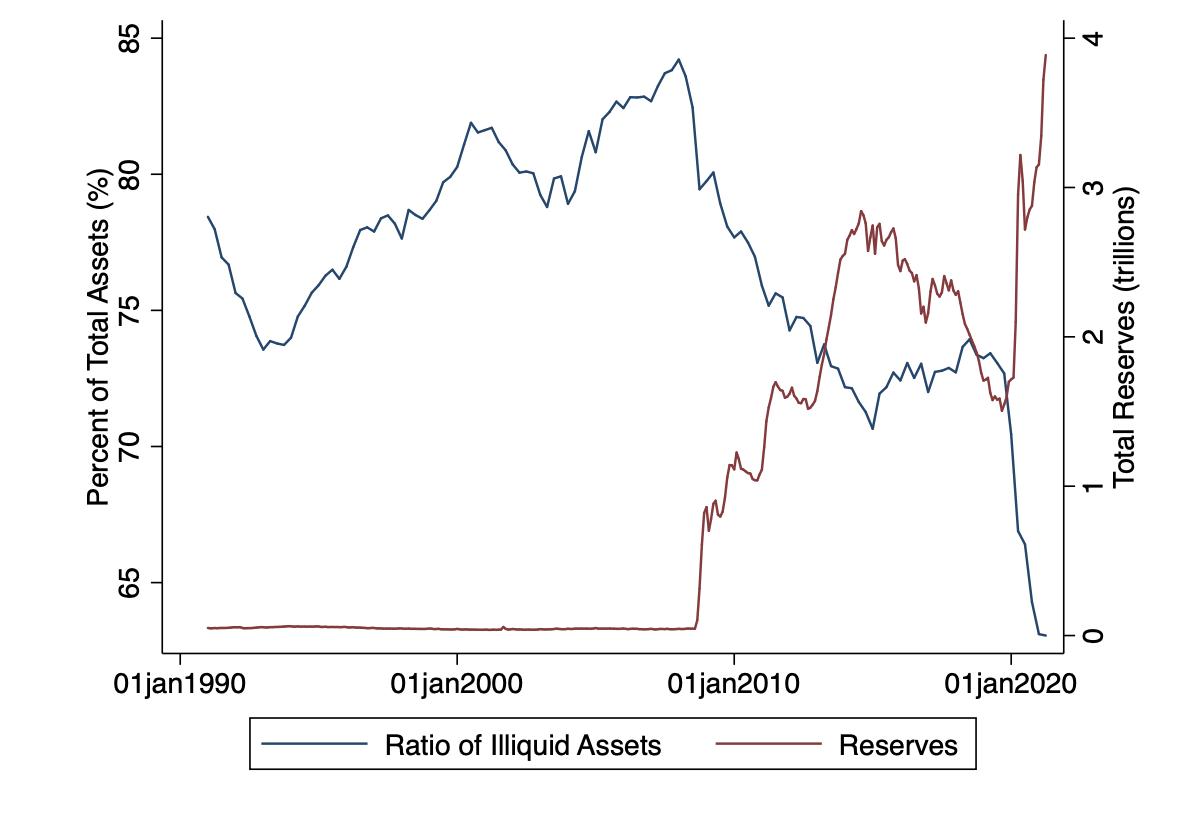
\includegraphics[width=.5\textwidth]{./imgs/motiv_supply_reserves_assets.png}
        \caption{Supply of Central Banks Reserves and Bank Asset Illiquidity}
        \end{figure}
        
      \end{frame}
    
\begin{frame}{Goal and Results}

\begin{wideitemize}
\item bla bla
\end{wideitemize}

    \end{frame}



\section{Related Literature}
\begin{frame}[label = lit]{Related Literature}

  \begin{wideitemize}
      \item 
      
      \begin{itemize}
        \item 
        \item 
      \end{itemize}


          \item Structural models of deposit competition

          \begin{itemize}
            \item 
            \item 
            \item 
          \end{itemize}
      
      \item 
      
      \begin{itemize}
          \item 
          \item 
      \end{itemize}

  \end{wideitemize}
  
\end{frame}

% \section{Background and Data}


% \begin{frame}[label = backg]{Background}



% \begin{itemize}
%     \item 
    
%     \item  \hyperlink{backg_col_diagram_appendix}{\beamergotobutton{C}}
%     \begin{itemize}
%         \item 
%     \end{itemize}
    
%     \item 
%     \end{itemize}

% \end{frame}


\begin{frame}{Data}

  Main data sources:
  \vspace{0.3cm}
\begin{wideitemize}
    \item  Summary of Deposits by FDIC (SOD)
    
    \begin{itemize}
      \item yearly as of June 30th. 
      \item commercial banks and thrifts FDIC insured
        \item quantity of deposits by branch 
        \item location by branch
    \end{itemize}
    \vspace{0.3cm}
    \item RateWatch (RW)
    
    \begin{itemize}
        \item Weakly survey over 100000 branches
        \item commercial banks, credit unions, thrifts
        \item Rates (APR and APY), FDIC identifier, geographic information
        \item products (e.g. savings, CD, MM, etc.) by size and maturity (12-month CD min 10K)
        \item If the branch is rate setter
    \end{itemize}
    \item 

    \end{wideitemize}
\end{frame}



    \begin{frame}{Data}

    Additional data sources:
    \vspace{0.3cm}
    \begin{wideitemize}
      \item Call Reports and Thrift Financial Reports (Call Reports)
        
      \begin{itemize}
          \item income statement, balance sheet, loans, deposits, investments,  bank's capital, asset sale information
          \item bank characteristics: number of employees
        
          
      \end{itemize}

      \item The Financial Performance Reports and National Credit Union Association
        \begin{itemize}
          \item deposits 
      \end{itemize}
    \end{wideitemize}

  \end{frame}


% \begin{frame}{Descriptive Statistics}

%   After RW and SOD match:
%   \begin{table}[h]
%   \import{tables/}{general.tex}
%   \end{table}

%   \begin{itemize}
%     \item Including local banks
%   \end{itemize}
% \end{frame}


% \begin{frame}{Descriptive Statistics: Market Level}

%   %\textbf{Market level:}

%   \begin{table}[h]
%   \import{tables/}{mkt_tab.tex}
%   \end{table}

%   %\vspace(0.5cm)
%   \begin{itemize}
%     \item Only local banks in outside option
%     \item Credit unions are missing from outside option (around 8\% share in 2020)
%   \end{itemize}

% \end{frame}





\begin{frame}
    \textcolor{blue}{\huge{\centerline{Model of Bank Balance Sheets}}}

\end{frame}
    
\begin{frame}{Model}
    \vspace{0.3cm}
    Bank $m$ choose rates and security quantities at time $t$ to maximize the expected present value of its profits at time $t+1$ in all markets $n$:
    \begin{equation}
        \begin{gathered}
        \max _{\left(R_{D, n m t}, R_{M, n m t}, R_{L, n m t}, Q_{S, m t}\right)} \sum_n Q_{L, n m t}\left(R_{L, n m t}-R_t^{L, m}\right)+\sum_n Q_{M, n m t}\left(R_{M, n m t}-R_t^{L, m}\right) \\
        +Q_{S, m t}\left(R_{S, t}-R_t^{S, m}\right)-\sum_n Q_{D, n m t}\left(R_{D, n m t}-R_t^{D, m}\right)-C\left(\Theta_{m t}\right)
        \end{gathered}
        \end{equation}
        \vspace{0.1cm}
        \begin{itemize}
            \item $R_{D,nmt}$, $R_{M,nmt}$, $R_{L,nmt}$ are bank deposit, mortgages, and loan rates.
            \item $R_{S,t}$ is the security rate in the competitive market. 
            \item $R^{D,m}_t$, $R^{M,m}_t$, $R^{L,m}_t$, $R^{S,m}_t$ are the cash flows discount rates of the deposits, mortgages, loans, and securities.
            \item $Q_{D, n m t}$,  $Q_{M, n m t}$,$Q_{L, n m t}$, $Q_{S, m t}$ are the quantities of deposits, mortgages, loans, and securities.
            \item $C(\Theta_{mt})$ is the balance sheet costs ($\Theta_{mt}$ is the vector ($Q_{L, n m t}$, $Q_{M, n m t}$, $Q_{S, m t}$, $Q_{D, n m t}$))
    
            
        \end{itemize}
    \end{frame}
    
\begin{frame}{Model}

    The first order conditions of bank profits with respect to the choice variables, $R_{D, n m t}, R_{M, n m t}, R_{L, n m t}$, and $Q_{S, m t}$, are
    $$
    \begin{aligned}
        R_t^{D, m}-R_{D, n m t}-\frac{Q_{D, n m t}}{\partial Q_{D, n m t} / \partial R_{D, n m t} }& =  \frac{\partial C\left(\Theta_{m t}\right)}{\partial Q_{D, n m t}} \\
        R_{j, n m t}- R_t^{j, m} +\frac{Q_{j, n m t}}{\partial Q_{j, n m t} / \partial R_{j, n m t}} & =  \frac{\partial C\left(\Theta_{m t}\right)}{\partial Q_{j, n m t}}, \quad j \in \{ L,M,S \}\\
    % \overbrace{\frac{\partial}{\partial R_{D, n m t}}\left[Q_{D, n m t}\left(R_t^{D, m}-R_{D, n m t}\right)\right]}^{\text {Marginal Revenue }} & =\overbrace{\frac{\partial C\left(\Theta_{m t}\right)}{\partial Q_{D, n m t}} \frac{\partial Q_{D, n m t}}{\partial R_{D, n m t}}}^{\text {Marginal Cost }}, \\
    % \frac{\partial}{\partial R_{j, n m t}}\left[Q_{j, n m t}\left(R_{j, n m t}-R_t^{j, m}\right)\right] & =\frac{\partial C\left(\Theta_{m t}\right)}{\partial Q_{j, n m t}} \frac{\partial Q_{j, n m t}}{\partial R_{j, n m t}}, \quad j \in \{ L,M\} \} \\
    % \frac{\partial}{\partial R_{L, n m t}}\left[Q_{L, n m t}\left(R_{L, n m t}-R_t^{L, m}\right)\right] & =\frac{\partial C\left(\Theta_{m t}\right)}{\partial Q_{L, n m t}} \frac{\partial Q_{L, n m t}}{\partial R_{L, n m t}}, \\
    \underbrace{R_{S, t}-R_t^{S, m}}_{\text{Reserve spread}} & =\frac{\partial C\left(\Theta_{m t}\right)}{\partial Q_{S, m t}}.
    \end{aligned}
    $$

\end{frame}

\begin{frame}{Model}


    The comparative statics with respect to a change in bank $m$ 's liquid security holdings $Q_{S, m t}$ are
$$
\begin{aligned}
\frac{\partial\left(R_t^{D, m}-R_{D, n m t}-\frac{Q_{D, n m t}}{\partial Q_{D, n m t} / \partial R_{D, n m t}}\right)}{\partial Q_{D, n m t}} \frac{\partial Q_{D, n m t}}{\partial Q_{S, m t}} & =\frac{\partial^2 C\left(\Theta_{m t}\right)}{\partial Q_{D, n m t} \partial \Theta_{m t}} \cdot \frac{\partial \Theta_{m t}}{\partial Q_{S, m t}} \\
\frac{\partial\left(R_t^{j, m}-R_{j, n m t}-\frac{Q_{j, n m t}}{\partial Q_{j, n m t} / \partial R_{j, n m t}}\right)}{\partial Q_{j, n m t}} \frac{\partial Q_{j, n m t}}{\partial Q_{S, m t}} & =-\frac{\partial^2 C\left(\Theta_{m t}\right)}{\partial Q_{j, n m t} \partial \Theta_{m t}} \cdot \frac{\partial \Theta_{m t}}{\partial Q_{S, m t}}, \quad j \in \{ L,M\} \}  \\
% \frac{\partial\left(R_t^{L, m}-R_{L, n m t}-\frac{Q_{L, n m t}}{\partial Q_{L, n m t} / \partial R_{L, n m t}}\right)}{\partial Q_{L, n m t}} \frac{\partial Q_{L, n m t}}{\partial Q_{S, m t}} & =-\frac{\partial^2 C\left(\Theta_{m t}\right)}{\partial Q_{L, n m t} \partial \Theta_{m t}} \cdot \frac{\partial \Theta_{m t}}{\partial Q_{S, m t}} \\
% \frac{\partial Q_{S, m t}}{\partial Q_{S, m t}} & =1
\end{aligned}
$$
 where $\frac{\partial Q_{j, n m t}}{\partial Q_{S, m t}}$ is the response of each bank branch quantity of $j \in \{D,L,M \}$ % to a change in $Q_{S, m t}$, and $\frac{\partial \Theta_{m t}}{\partial Q_{S, m t}}$ is the response of the balance sheet costs to a change in $Q_{S, m t}$.
\end{frame}


\begin{frame}
    \textcolor{blue}{\huge{\centerline{Demand system}}}
\end{frame}


  
\begin{frame}{Motivation}
    \vspace{0.5cm}
      \begin{itemize}
        \item  bla
      \end{itemize}
      
        \begin{figure}[t*]
          \centering
    
          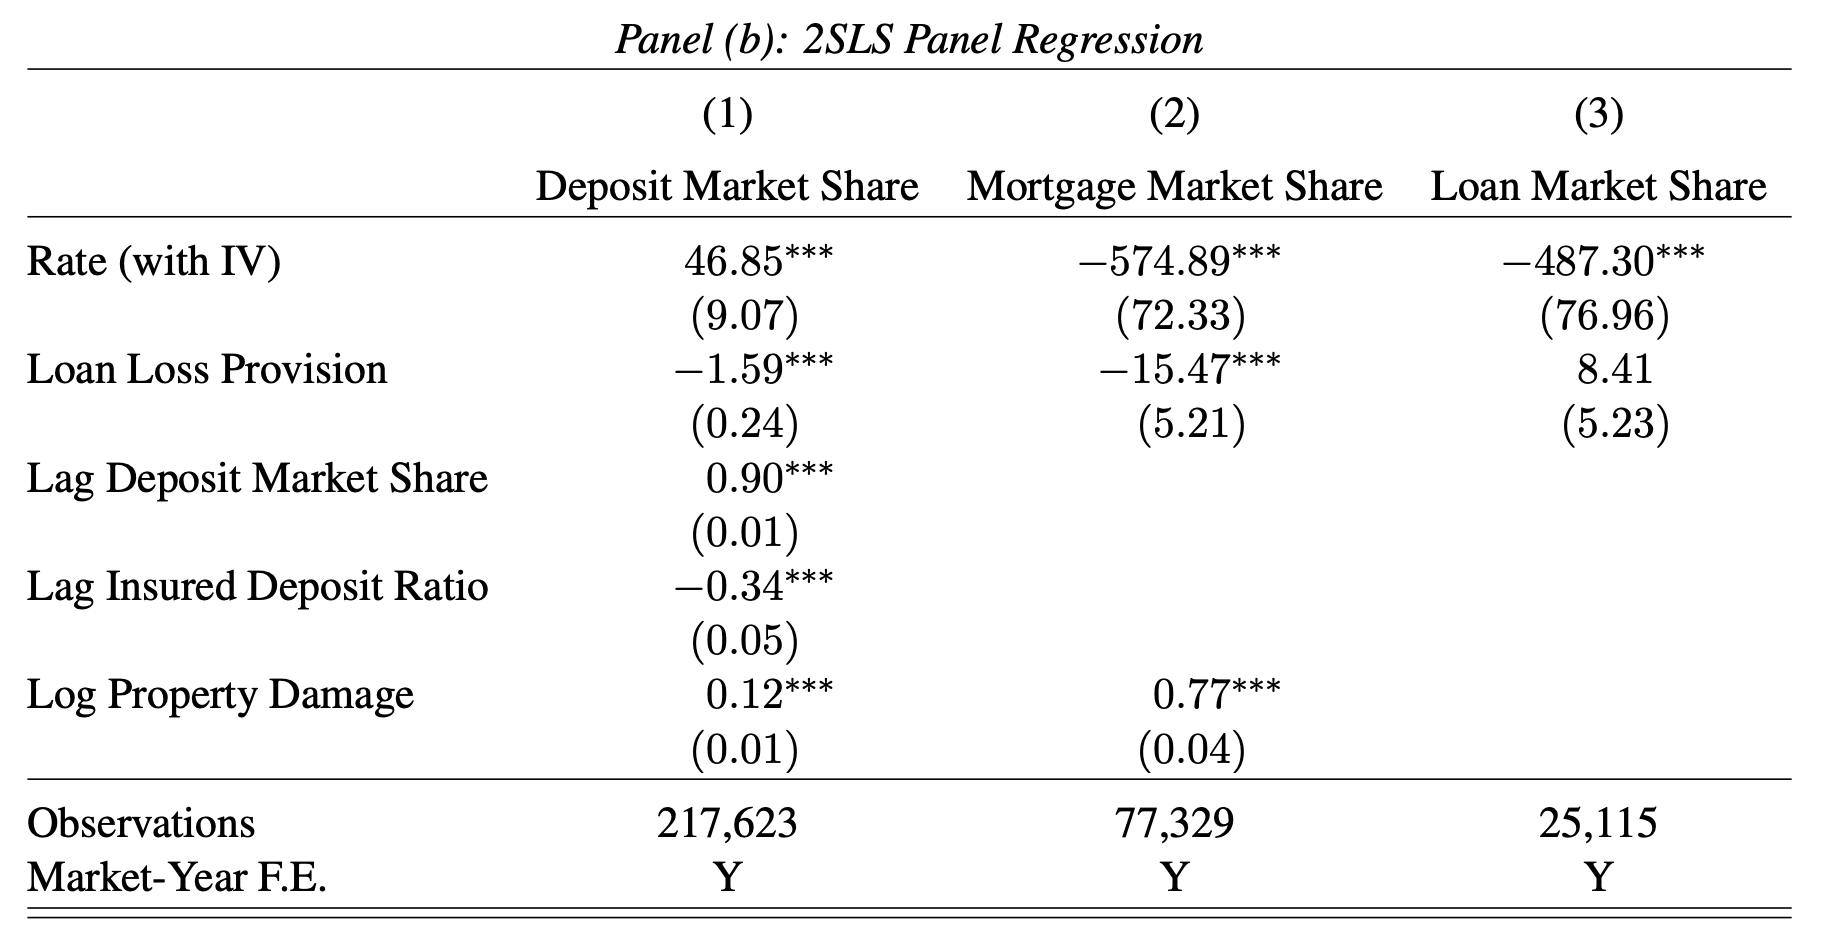
\includegraphics[width=.5\textwidth]{./imgs/second_stage_demand.png}
        % \caption{Supply of Central Banks Reserves and Bank Asset Illiquidity}
        \end{figure}
        
      \end{frame}

\begin{frame}
    \textcolor{blue}{\huge{\centerline{Cost function}}}
\end{frame}

\begin{frame}
    \textcolor{blue}{\huge{\centerline{Counterfactual}}}
\end{frame}


\begin{frame}
\textcolor{blue}{\huge{\centerline{Thank you!}}}
\end{frame}

%\section*{References}
%\begin{frame}{References}
%    \bibliographystyle{plainnat}
%    \bibliography{references.bib}
%\end{frame}


% \appendix


%  \begin{frame}[label=backg_data_appendix]{Appendix: Data Description \hyperlink{data}{\beamergotobutton{Back}}}
% \begin{itemize}
%   \item Product: SAV 2.5K (second most popular product)
%   \item Impute prices:
%   \item \begin{enumerate}
%     \item RateWatch data is missing some weeks (around 75\% of observations have missing weeks)
%     $$r_{jwt} = \text{ avg non-missing }_{jt} + \text{ fed rate$_w$ } + \text{ national avg$_{jw}$,} $$
%     \item From network of banks (rate setter) using RW.
%     \item Closest branch to the market centroid. 
%   \end{enumerate}
%   \item Drop bank-markets observations with less than 1\% rates.
%   \item Drop bank-markets observations with a single branch.
%   \item Local banks are defined as banks that get more than 90\% deposits from single market. 
% \end{itemize}
% \end{frame}


% \begin{frame}[label=backg_col_brack_appendix]{Appendix\hyperlink{backg}{\beamergotobutton{Back}}}

% \end{frame}

\end{document}